\documentclass[aspectratio=169,10pt]{beamer}
\usepackage[T1]{fontenc}
\usepackage[utf8]{inputenc}
\usepackage{lmodern}
\usepackage{amsmath,amssymb,booktabs,tabularx,array,graphicx}
\usepackage{ragged2e}
\usepackage{tikz}
\usepackage{pgfplots}
\usepackage{siunitx}
\pgfplotsset{compat=1.16}
\usetikzlibrary{shadows.blur,arrows.meta,positioning,calc}
\sisetup{
    output-decimal-marker={.},
    group-separator={,},
    group-digits=integer,
    range-phrase={--},
    range-units=single,
    detect-all,
    per-mode=symbol
}

\definecolor{navy}{HTML}{1C508C}
\definecolor{greenbox}{HTML}{127447}
\definecolor{redbox}{HTML}{B52B2E}
\definecolor{gold}{HTML}{F6BE16}
\definecolor{pale}{HTML}{F2F5F9}
\setbeamercolor{normal text}{fg=black,bg=white}
\setbeamercolor{frametitle}{fg=white,bg=navy}
\setbeamerfont{frametitle}{size=\large,series=\bfseries}
\setbeamercolor{structure}{fg=navy}
\setbeamercolor{block title}{fg=white,bg=navy}
\setbeamercolor{block body}{fg=black,bg=pale}
\setbeamercolor{block title alerted}{fg=white,bg=redbox}
\setbeamercolor{block body alerted}{fg=black,bg=redbox!5}
\setbeamercolor{block title example}{fg=white,bg=greenbox}
\setbeamercolor{block body example}{fg=black,bg=greenbox!5}
\setbeamertemplate{navigation symbols}{}
\setbeamertemplate{blocks}[rounded][shadow=true]
\setbeamertemplate{itemize items}[circle]
\setbeamertemplate{enumerate items}[circle]
\setbeamertemplate{frametitle}{\nointerlineskip\begin{beamercolorbox}[wd=\paperwidth,ht=0.70cm,dp=0.18cm,leftskip=.35cm]{frametitle}\usebeamerfont{frametitle}\insertframetitle\end{beamercolorbox}}
\setbeamercolor{footcenter}{fg=black,bg=gold}
\setbeamertemplate{footline}{\leavevmode\hbox{\begin{beamercolorbox}[wd=.31\paperwidth,ht=.34cm,dp=.14cm,center]{frametitle}\fontsize{7}{8}\selectfont Group I --- Physics UNAIR\end{beamercolorbox}\begin{beamercolorbox}[wd=.42\paperwidth,ht=.34cm,dp=.14cm,center]{footcenter}\fontsize{7}{8}\selectfont Instrumentation Calibration \& Metrology\end{beamercolorbox}\begin{beamercolorbox}[wd=.27\paperwidth,ht=.34cm,dp=.14cm,right]{frametitle}\fontsize{7}{8}\selectfont 17 Nov 2026\hspace{.22cm}\insertframenumber / \inserttotalframenumber\hspace{.2cm}\end{beamercolorbox}}}
\setbeamersize{text margin left=.37cm,text margin right=.37cm}

\newcommand{\sm}{\fontsize{8.2}{10.2}\selectfont}
\newcommand{\xs}{\fontsize{7.1}{9}\selectfont}
\newcommand{\capx}[1]{\par\vspace{1mm}{\centering\xs #1\par}}
\newcommand{\uc}{u_{c}}
\newcommand{\uA}{u_{A}}
\newcommand{\uB}{u_{B}}

\title{INSTRUMENTATION CALIBRATION AND METROLOGICAL EVALUATION}
\subtitle{Case-Based Elaborative Project: Experiments P1 (Density) and M3 (Energy)}
\author{Muhammad Abiyu Khansa \and Farras Atha Pandita \and Hendra Maulana}
\date{17 November 2026}

\begin{document}

%=============================================================================
% FRAME 1: TITLE SLIDE
%=============================================================================
\begin{frame}[plain]
\centering
\vspace*{0.1cm}
\begin{beamercolorbox}[wd=\linewidth,sep=8pt,center,rounded=true,shadow=true]{frametitle}
  {\Large\bfseries INSTRUMENTATION CALIBRATION AND METROLOGICAL EVALUATION\par}
  \vspace{1.5mm}
  {\normalsize\normalfont Case-Based Elaborative Project --- Experiments P1 (\textit{Density}) and M3 (\textit{Energy})\par}
\end{beamercolorbox}

\vspace{0.3cm}

\includegraphics[height=2.2cm,keepaspectratio]{Images/logo-unair.png}
\vspace{0.25cm}

{\sm\textbf{Prepared by (Group I):}\par}
\vspace{1mm}
{\sm Muhammad Abiyu Khansa (182241036) \quad Farras Atha Pandita (182241040) \quad Hendra Maulana (182241043)\par}
\vspace{2mm}
{\xs\textbf{Faculty Supervisor:} Yhosep Gita Yhun Yhuwana, S.Si., M.T.\par}
\vspace{1.5mm}
{\xs Department of Physics, Faculty of Science and Technology, Universitas Airlangga\par}
\vspace{1mm}
{\xs 17 November 2026\par}
\vfill
\end{frame}

%=============================================================================
% FRAME 2: TABLE OF CONTENTS
%=============================================================================
\begin{frame}{Outline}\tableofcontents[hideallsubsections]\end{frame}

%=============================================================================
% SECTION 1: OVERVIEW AND OBJECTIVES
%=============================================================================
\section{Overview and Objectives}

\begin{frame}{Executive Summary and Key Metrological Findings}
\begin{columns}[T,onlytextwidth]
\begin{column}{.49\textwidth}
\begin{block}{Project Scope}\sm
\begin{itemize}
\item Metrological evaluation ($n=8$ repeated trials) on paired benchmark experiments: \textbf{P1 (brass cylinder density)} and \textbf{M3 (air-track mechanical energy)}.
\item $3\sigma$ outlier screening retained 100\% of measurements.
\item Uncertainty evaluation via \textbf{ISO-GUM} ($\uA$, $\uB$, $\uc$, and expanded $U$ at $k=2$).
\item 8-point OLS balance calibration against Class F2 weights ($10\text{--}300\text{ g}$).
\end{itemize}
\end{block}
\begin{exampleblock}{Primary P1 \& Calibration Results}\sm
$\rho = (8.493 \pm 0.035)\ \si{g/cm^3}$ (diameter drives $85.4\%$ of variance); OLS fit $y = 0.999975\,x + 0.0421\ \si{g}$ ($R^2 \approx 1$).
\end{exampleblock}
\end{column}

\begin{column}{.49\textwidth}
\begin{block}{Quantitative M3 Findings}\sm
\begin{itemize}
\item \textbf{Measured velocities:} $v_1 = (0.4798 \pm 0.0016)\ \si{m/s}$, $v_2 = (0.8985 \pm 0.0033)\ \si{m/s}$.
\item \textbf{Initial energy ($E_1$):} $(0.07798 \pm 0.00022)\ \si{J}$.
\item \textbf{Final energy ($E_2$):} $(0.08077 \pm 0.00060)\ \si{J}$.
\item \textbf{Energy discrepancy ($\Delta E = E_1 - E_2$):}
  $$\Delta E = (-2.79 \pm 0.61) \times 10^{-3}\ \si{J}.$$
\end{itemize}
\end{block}
\begin{alertblock}{Critical Insight}\sm
$\Delta E < 0$ ($E_2 > E_1$) is not a conservation violation, but a signature of \textbf{dynamic systematic error} (photogate latency $\tau$), alongside curved balance residuals ($e_{\max} = 0.032\ \si{g}$).
\end{alertblock}
\end{column}
\end{columns}
\end{frame}

\begin{frame}{Background, Problem Statements, and Objectives}
\begin{columns}[T,onlytextwidth]
\begin{column}{.49\textwidth}
\begin{block}{Background}\xs
\begin{itemize}
\item Deployment of a new batch of lab instruments (digital balances, vernier calipers, air track with photogates) revealed inter-instrument deviations.
\item Potential sources: hysteresis, mechanical friction, \textit{modifying inputs}, \textit{noise}, \textit{loading effects}, and digital resolution limits.
\item Goal: isolate whether deviations stem from instrument defects, calibration offsets, or random noise.
\end{itemize}
\end{block}
\begin{exampleblock}{Objectives}\xs
\begin{enumerate}
\item Map static \& dynamic instrument performance metrics.
\item Execute OLS calibration $y=ax+b$ and residual checks.
\item Propagate $\uA, \uB, \uc, U$ ($k=2$) per ISO-GUM.
\end{enumerate}
\end{exampleblock}
\end{column}

\begin{column}{.49\textwidth}
\begin{block}{Core Research Questions}\xs
\begin{enumerate}
\item What are the static and dynamic performance characteristics in P1 and M3?
\item Does OLS calibration against Class F2 weights confirm true linearity?
\item What are $\uc$ and $U$ ($k=2$) for brass density $\rho$ and energy loss $\Delta E$?
\item How do instrumental limitations impact physical conclusions?
\end{enumerate}
\end{block}
\begin{alertblock}{Experimental Design ($n=8$)}\xs
Following the 3-member group protocol, repetitions were reduced by $25\%$ to $n=8$ trials per measurand while preserving full analytical rigor.
\end{alertblock}
\end{column}
\end{columns}
\end{frame}

%=============================================================================
% SECTION 2: EXPERIMENTAL METHODS AND DATA
%=============================================================================
\section{Experimental Methods and Data}

\begin{frame}{Instrument Specifications and Experimental Setup}
\begin{columns}[T,onlytextwidth]
\begin{column}{.50\textwidth}
\begin{block}{Evaluated Instrument Profile}\xs
\begin{tabular}{@{}lll@{}}
\toprule
\textbf{Exp.} & \textbf{Instrument} & \textbf{Resolution}\\
\midrule
P1 & Digital balance (0--500 g) & \SI{0.01}{g}\\
P1/M3 & Vernier caliper ($d, h, w$) & \SI{0.05}{mm}\\
M3 & Height gauge ($\Delta h$) & \SI{0.1}{mm}\\
M3 & Photogate + digital \textit{timer} & \SI{0.1}{ms}\\
Cal. & Class F2 standard weights & $u_{\mathrm{std}} \le \SI{0.002}{g}$\\
\bottomrule
\end{tabular}
\end{block}
\begin{exampleblock}{Governing Equations}\sm
$$\rho = \frac{4m}{\pi d^2 h}, \qquad v_i = \frac{w}{\Delta t_i}$$
$$E_1 = \tfrac{1}{2}Mv_1^2 + Mg\Delta h, \quad E_2 = \tfrac{1}{2}Mv_2^2$$
\end{exampleblock}
\end{column}

\begin{column}{.48\textwidth}
\centering
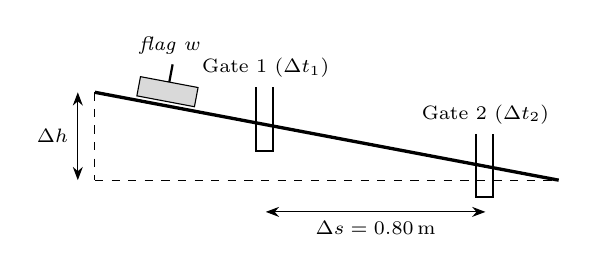
\begin{tikzpicture}[>=Stealth,scale=0.62]
  \draw[very thick] (0,2.2) -- (9.5,0.4);
  \draw[dashed] (0,0.4) -- (9.5,0.4);
  \draw[dashed] (0,2.2) -- (0,0.4);
  \draw[<->] (-0.35,0.4) -- (-0.35,2.2) node[midway,left]{\xs $\Delta h$};
  \begin{scope}[rotate=-10.7,shift={(0.45,2.2)}]
    \fill[gray!30,draw=black] (0,0.05) rectangle (1.2,0.45);
    \draw[thick] (0.60,0.45) -- (0.60,0.82);
    \node[above] at (0.55,0.82) {\xs \textit{flag} $w$};
  \end{scope}
  \draw[thick] (3.3,2.3) -- (3.3,1.0) -- (3.65,1.0) -- (3.65,2.3);
  \node[above] at (3.5,2.3) {\xs Gate 1 ($\Delta t_1$)};
  \draw[thick] (7.8,1.35) -- (7.8,0.05) -- (8.15,0.05) -- (8.15,1.35);
  \node[above] at (8.0,1.35) {\xs Gate 2 ($\Delta t_2$)};
  \draw[<->] (3.5,-0.25) -- (8.0,-0.25) node[midway,below]{\xs $\Delta s=\SI{0.80}{m}$};
\end{tikzpicture}
\capx{Figure 1. M3 inclined air-track schematic ($g=\SI{9.806}{m/s^2}$, $\Delta h \approx \SI{28}{mm}$).}
\begin{block}{Screening Protocol}\xs
All raw readings were logged without pre-rounding and screened via $|x_i-\bar{x}| > 3\sigma$.
\end{block}
\end{column}
\end{columns}
\end{frame}

\begin{frame}{Raw Datasets ($n=8$) and $3\sigma$ Outlier Screening}
\begin{columns}[T,onlytextwidth]
\begin{column}{.53\textwidth}
\begin{block}{Raw Measurements (8 Trials)}\xs
\centering
\begin{tabular}{@{}ccccccc@{}}
\toprule
\textbf{Tr.} & $m$ (g) & $d$ (mm) & $h$ (mm) & $\Delta t_1$ (s) & $\Delta t_2$ (s) & $M$ (g)\\
\midrule
1 & 67.22 & 20.05 & 25.10 & 0.0521 & 0.0278 & 200.10\\
2 & 67.21 & 20.00 & 25.15 & 0.0519 & 0.0279 & 200.12\\
3 & 67.23 & 20.05 & 25.10 & 0.0523 & 0.0277 & 200.08\\
4 & 67.20 & 20.10 & 25.05 & 0.0520 & 0.0280 & 200.11\\
5 & 67.24 & 20.00 & 25.10 & 0.0522 & 0.0278 & 200.09\\
6 & 67.22 & 20.05 & 25.15 & 0.0518 & 0.0279 & 200.10\\
7 & 67.21 & 20.00 & 25.10 & 0.0524 & 0.0277 & 200.13\\
8 & 67.23 & 20.05 & 25.05 & 0.0521 & 0.0278 & 200.07\\
\bottomrule
\end{tabular}
\par\vspace{1mm}
{\xs Mean flag width $w \approx 25.00\ \si{mm}$ and elevation $\Delta h \approx 28.0\ \si{mm}$.}
\end{block}
\end{column}

\begin{column}{.45\textwidth}
\begin{exampleblock}{Max Standardized Deviation ($z_{\max}$)}\xs
\centering
\begin{tabular}{@{}lcc@{}}
\toprule
\textbf{Quantity} & $z_{\max}$ & \textbf{Result ($<3$)}\\
\midrule
Mass $m$ (P1) & 1.53 & All pass\\
Diameter $d$ & 1.77 & All pass\\
Height $h$ & 1.32 & All pass\\
Time $\Delta t_1$ & 1.50 & All pass\\
Time $\Delta t_2$ & 1.69 & All pass\\
Mass $M$, $w$, $\Delta h$ & 1.50 / 1.32 & All pass\\
\bottomrule
\end{tabular}
\end{exampleblock}
\begin{alertblock}{Small-Sample Limitation}\xs
For $n=8$, the mathematical upper bound is $(n-1)/\sqrt{n} \approx 2.47 < 3$. Thus $3\sigma$ cannot flag outliers on $n=8$ using sample $s$; data quality is instead evidenced by tight standard deviations.
\end{alertblock}
\end{column}
\end{columns}
\end{frame}

%=============================================================================
% SECTION 3: STATIC AND DYNAMIC CHARACTERISTICS
%=============================================================================
\section{Static and Dynamic Characteristics}

\begin{frame}{Static Instrument Characteristics (Experiment P1)}
\begin{columns}[T,onlytextwidth]
\begin{column}{.49\textwidth}
\begin{block}{Accuracy, Precision, and Repeatability}\sm
\begin{itemize}
\item \textbf{Accuracy (vs. $\SI{67.20}{g}$ ref.):}
  $$E_{\mathrm{abs}} = \SI{0.020}{g}, \quad E_{\mathrm{rel}} = 2.98\times 10^{-4}\ (0.030\%).$$
\item Bias $\SI{0.020}{g} > U_m = \SI{0.011}{g}$ $\implies$ metrologically significant.
\item \textbf{Precision \& Repeatability:} $s_r = \SI{0.0131}{g}$, $r = 2.8\,s_r = \SI{0.037}{g}$.
\item \textbf{OLS Sensitivity:} $S = 0.999975\ \si{g/g}$ (ideal $1.000000$).
\end{itemize}
\end{block}
\end{column}

\begin{column}{.49\textwidth}
\begin{exampleblock}{No-Load \textit{Zero Drift} Test (30 min)}\sm
\centering
\setlength{\tabcolsep}{3.5pt}\begin{tabular}{@{}lccccccc@{}}
\toprule
\textbf{Min} & 0 & 5 & 10 & 15 & 20 & 25 & 30\\
\midrule
\textbf{Zero (g)} & 0.00 & 0.00 & 0.01 & 0.01 & 0.02 & 0.02 & 0.03\\
\bottomrule
\end{tabular}
\par\vspace{2mm}\raggedright
\begin{itemize}
\item $+\SI{0.03}{g}$ drift over $30$ min ($\approx \SI{1e-3}{g/min}$), equal to $3\times$ resolution.
\item Attributed to strain-gauge mechanical \textit{creep} and thermal ADC drift.
\end{itemize}
\end{exampleblock}
\begin{alertblock}{Operational Mitigation}\xs
The digital balance must be re-zeroed (\textit{tare}) prior to every measurement series.
\end{alertblock}
\end{column}
\end{columns}
\end{frame}

\begin{frame}{Dynamic Characteristics and Loading Effects (Experiment M3)}
\begin{columns}[T,onlytextwidth]
\begin{column}{.50\textwidth}
\begin{block}{Photogate \textit{Response Time Delay} ($\tau$)}\sm
Comparator hysteresis creates delay $\Delta t_{\mathrm{meas}} = \Delta t_{\mathrm{true}} - \tau$. Assuming $\tau = \SI{0.8}{ms}$:
\par\vspace{1.5mm}\centering\xs
\setlength{\tabcolsep}{3.5pt}\begin{tabular}{@{}lccc@{}}
\toprule
\textbf{Gate} & $v_{\mathrm{meas}}$ (m/s) & $v_{\mathrm{corr}}$ (m/s) & \textbf{Bias (\%)}\\
\midrule
1 ($\overline{\Delta t_1} = \SI{52.10}{ms}$) & 0.4798 & 0.4726 & 1.54\\
2 ($\overline{\Delta t_2} = \SI{27.825}{ms}$) & 0.8985 & 0.8734 & 2.88\\
\bottomrule
\end{tabular}
\par\vspace{1.5mm}\raggedright\sm
Gate~2 bias is nearly double Gate~1 because $\tau/\Delta t_2 > \tau/\Delta t_1$ (systematic error).
\end{block}
\end{column}

\begin{column}{.48\textwidth}
\begin{exampleblock}{\textit{Loading Effect} (Th\'evenin Analogy)}\sm
$$\frac{E_m}{E_o} = \frac{R_m}{R_{AB} + R_m}$$
Boundary-layer air friction and passive eddy-current damping act analogously to internal impedance $R_{AB}$ dissipating mechanical energy.
\end{exampleblock}
\begin{alertblock}{Environmental \textit{Modifying Inputs}}\sm
\begin{itemize}
\item HVAC airflow alters aerodynamic drag on the \textit{glider}.
\item Minor track-level non-uniformity shifts the effective elevation $\Delta h$.
\end{itemize}
\end{alertblock}
\end{column}
\end{columns}
\end{frame}

%=============================================================================
% SECTION 4: ISO-GUM UNCERTAINTY EVALUATION
%=============================================================================
\section{ISO-GUM Uncertainty Evaluation}

\begin{frame}{ISO-GUM Uncertainty Budget for P1 (Brass Density $\rho$)}
\begin{columns}[T,onlytextwidth]
\begin{column}{.49\textwidth}
\begin{block}{ISO-GUM Equations \& Direct Inputs}\xs
$$\uA = \frac{s}{\sqrt{n}}, \quad \uB = \frac{\Delta x}{2\sqrt{3}}, \quad \uc = \sqrt{\uA^2+\uB^2}, \quad U = 2\uc$$
\centering
\setlength{\tabcolsep}{3.5pt}\begin{tabular}{@{}lccc@{}}
\toprule
\textbf{Parameter} & $m$ (g) & $d$ (cm) & $h$ (cm)\\
\midrule
Mean $\bar{x}$ & 67.22000 & 2.00375 & 2.51000\\
$\uA$ & 0.00463 & 0.00125 & 0.00134\\
$\uB$ & 0.00289 & 0.00144 & 0.00144\\
$\uc$ & 0.00546 & 0.00191 & 0.00197\\
$U = 2\uc$ & 0.01091 & 0.00382 & 0.00393\\
\bottomrule
\end{tabular}
\end{block}
\end{column}

\begin{column}{.49\textwidth}
\begin{exampleblock}{Density Uncertainty Budget}\xs
\centering
\begin{tabular}{@{}lcc@{}}
\toprule
\textbf{Source} & \textbf{Contrib. to $\uc(\rho)/\rho$} & \textbf{Variance (\%)}\\
\midrule
Mass $m$ & 0.00008 & 0.2\\
Diameter $d$ ($\times 2$) & 0.00191 & \textbf{85.4}\\
Height $h$ & 0.00078 & 14.4\\
\midrule
\textbf{Combined} & \textbf{0.00206} & \textbf{100.0}\\
\bottomrule
\end{tabular}
\par\vspace{2mm}\sm
$$\boxed{\rho = (8.493 \pm 0.035)\ \si{g/cm^3}\ (k=2), \quad \frac{U}{\rho}=0.41\%}$$
\end{exampleblock}
\begin{alertblock}{Key Takeaway (P1)}\xs
Consistent with brass ($\approx 8.4\text{--}8.7\ \si{g/cm^3}$). Diameter drives $85.4\%$ of variance due to the caliper's $\SI{0.05}{mm}$ resolution.
\end{alertblock}
\end{column}
\end{columns}
\end{frame}

\begin{frame}{ISO-GUM Uncertainty Propagation for M3 ($\Delta E$)}
\begin{columns}[T,onlytextwidth]
\begin{column}{.50\textwidth}
\begin{block}{Direct Inputs \& Variance Share}\xs
\centering
\setlength{\tabcolsep}{3.5pt}\begin{tabular}{@{}lccc@{}}
\toprule
\textbf{Quantity} & \textbf{Mean} & $\uc$ & \textbf{$\Delta E$ Var. (\%)}\\
\midrule
$\Delta t_2$ (s) & 0.027825 & $4.66\times 10^{-5}$ & \textbf{79.6}\\
$w$ (m) & 0.025000 & $1.97\times 10^{-5}$ & 9.0\\
$\Delta h$ (m) & 0.028000 & $3.93\times 10^{-5}$ & 6.5\\
$\Delta t_1$ (s) & 0.052100 & $7.64\times 10^{-5}$ & 5.0\\
$M$ (kg) & 0.200100 & $7.64\times 10^{-6}$ & 0.0\\
\bottomrule
\end{tabular}
\par\vspace{1.5mm}\raggedright
Because $E_1$ and $E_2$ share $M$ and $w$, correlated propagation was computed via symbolic partial derivatives in \texttt{SymPy}.
\end{block}
\end{column}

\begin{column}{.48\textwidth}
\begin{exampleblock}{Mechanical Energy Results ($k=2$)}\sm
\begin{itemize}
\item $E_{k1} = \SI{0.02304}{J}$, \quad $E_{p1} = \SI{0.05494}{J}$
\item $E_1 = (0.07798 \pm 0.00022)\ \si{J}$
\item $E_2 = (0.08077 \pm 0.00060)\ \si{J}$
\item $\boxed{\Delta E = (-2.79 \pm 0.61)\times 10^{-3}\ \si{J}}$
\end{itemize}
{\xs (Uncorrelated $U(\Delta E)=\SI{0.00064}{J}$ leaves conclusions unchanged.)}
\end{exampleblock}
\begin{alertblock}{Physical Anomaly ($\Delta E < 0$)}\xs
$\Delta E$ lies $\approx 4.6\,U$ below zero, implying an apparent energy gain—evidence of uncompensated systematic bias exceeding $U(\Delta E)$.
\end{alertblock}
\end{column}
\end{columns}
\end{frame}

%=============================================================================
% SECTION 5: CALIBRATION AND VALIDATION
%=============================================================================
\section{OLS Calibration and Residual Analysis}

\begin{frame}{Digital Balance Calibration and Linearity Assessment}
\begin{columns}[T,onlytextwidth]
\begin{column}{.48\textwidth}
\begin{block}{8-Point Class F2 Calibration Data}\xs
\centering
\begin{tabular}{@{}cccc@{}}
\toprule
\textbf{Std $x$ (g)} & \textbf{Read $y$ (g)} & $\hat{y}$ \textbf{(g)} & \textbf{Residual $e_i$ (g)}\\
\midrule
10.00 & 10.02 & 10.0419 & $-0.0219$\\
20.00 & 20.03 & 20.0416 & $-0.0116$\\
50.00 & 50.04 & 50.0409 & $-0.0009$\\
100.00 & 100.06 & 100.0396 & $+0.0204$\\
150.00 & 150.07 & 150.0384 & $+0.0316$\\
200.00 & 200.05 & 200.0371 & $+0.0129$\\
250.00 & 250.03 & 250.0359 & $-0.0059$\\
300.00 & 300.01 & 300.0346 & $-0.0246$\\
\bottomrule
\end{tabular}
\end{block}
\end{column}

\begin{column}{.50\textwidth}
\begin{exampleblock}{OLS Regression Fit}\sm
$$\boxed{y = 0.999975\,x + 0.0421\ \si{g}, \quad R^2 = 0.99999997}$$
\begin{itemize}
\item $s_{y/x} = \SI{0.0217}{g}$, $u(a)=7.6\times 10^{-5}$, $u(b)=\SI{0.013}{g}$.
\item $|a-1| < u(a)$ $\implies$ sensitivity matches unity.
\item Intercept $b = \SI{0.042}{g}$ ($\approx 3.3\,u(b)$) aligns with observed \textit{zero drift} ($\SI{0.03}{g}$).
\end{itemize}
\end{exampleblock}
\begin{alertblock}{Why $R^2 \approx 1$ Is Insufficient}\xs
A quadratic model lowers $s_{y/x}$ to $\SI{0.0056}{g}$ ($c_2 = -2.3\times 10^{-6}\ \si{g^{-1}}$). Despite $R^2 \approx 1$, residuals form an inverted parabolic arc (max $\SI{0.032}{g}$).
\end{alertblock}
\end{column}
\end{columns}
\end{frame}

\begin{frame}{Calibration Curve, Residual Pattern, and Validation Tests}
\begin{columns}[T,onlytextwidth]
\begin{column}{.56\textwidth}
\centering
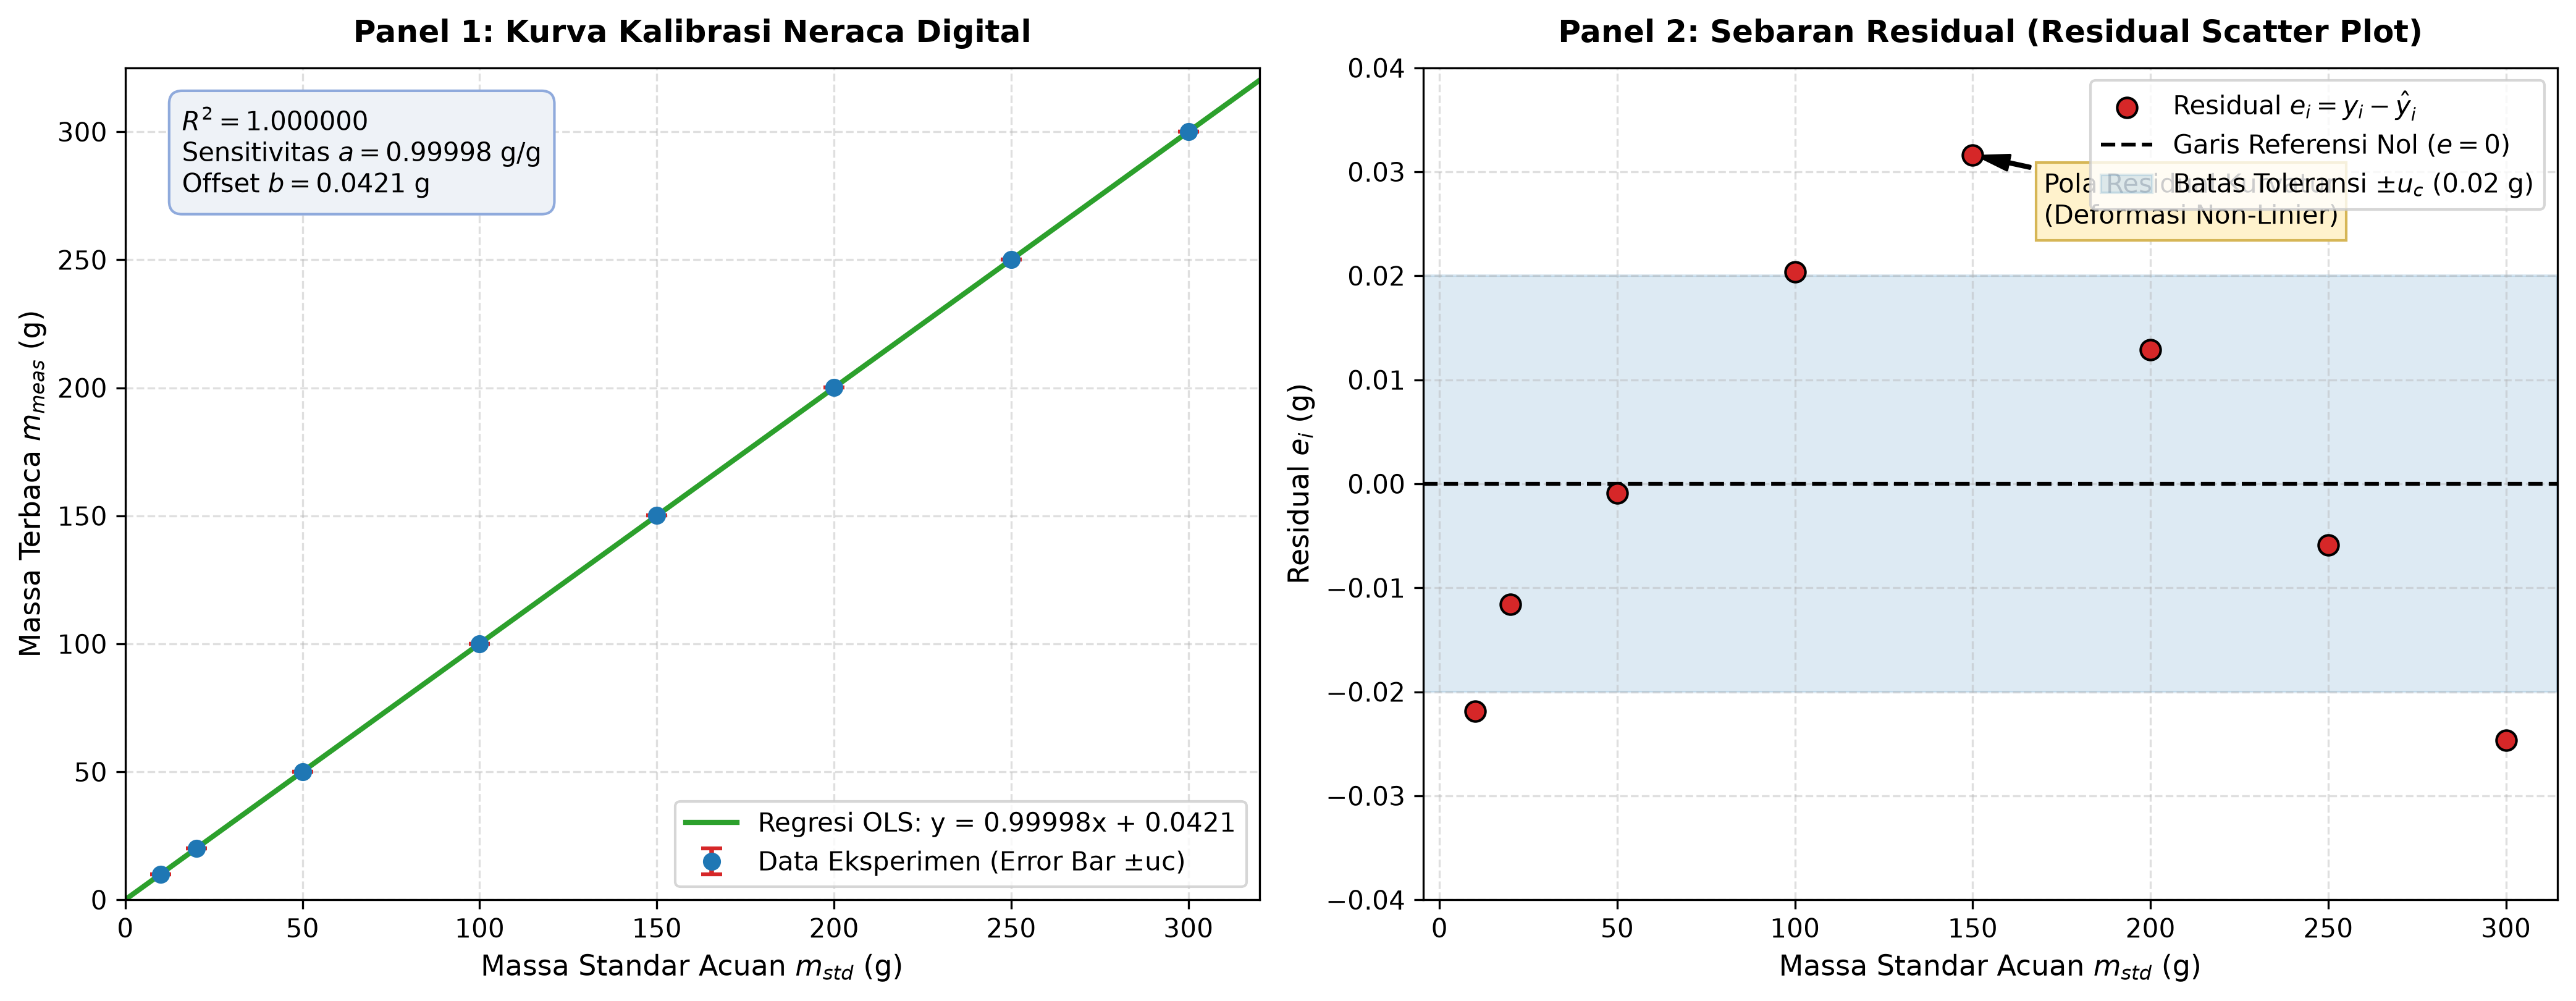
\includegraphics[width=\linewidth,keepaspectratio]{Images/Kalibrasi_Residual.png}
\capx{Figure 2. OLS calibration line (left) vs. non-random curved residual pattern (right).}
\end{column}

\begin{column}{.42\textwidth}
\begin{block}{Summary of 5 Validation Tests}\xs
\begin{enumerate}
\item \textbf{Accuracy:} P1 bias $\SI{0.020}{g}$ ($> U_m$); peak calibration error $+\SI{0.07}{g}$ at $\SI{150}{g}$.
\item \textbf{Repeatability:} $s_r=\SI{0.0131}{g}$, $r=\SI{0.037}{g}$ ($\approx 1$ digit).
\item \textbf{Linearity:} Max deviation $\SI{0.032}{g}$ ($0.011\%$ FS), curved pattern.
\item \textbf{Functional:} Stable to $2$ decimals; periodic \textit{zeroing} required.
\item \textbf{Response/Stability:} \textit{Zero drift} $+\SI{0.03}{g}/30$ min; assumed gate delay $\approx \SI{0.8}{ms}$.
\end{enumerate}
\end{block}
\end{column}
\end{columns}
\end{frame}

%=============================================================================
% SECTION 6: DISCUSSION, CONCLUSIONS, AND REFERENCES
%=============================================================================
\section{Discussion, Conclusions, and References}

\begin{frame}{Reflective ``So What?'' Analysis: Root-Cause Diagnosis}
\begin{columns}[T,onlytextwidth]
\begin{column}{.48\textwidth}
\begin{block}{Experiment P1 (Static Metrology)}\sm
\begin{itemize}
\item $\rho = (8.493 \pm 0.035)\ \si{g/cm^3}$ identifies the specimen as brass, though $0.41\%$ cannot distinguish Cu--Zn alloy grades.
\item Replacing the caliper ($\SI{0.05}{mm}$) with a micrometer ($\SI{0.01}{mm}$) for $d$ cuts $U(\rho)$ down to $\sim \SI{0.026}{g/cm^3}$—far better than adding mass trials.
\end{itemize}
\end{block}
\begin{exampleblock}{Static vs. Dynamic Regimes}\xs
P1 is bounded by random/resolution noise, whereas M3 is dominated by systematic latency $\tau$ that evades $3\sigma$ checks.
\end{exampleblock}
\end{column}

\begin{column}{.50\textwidth}
\begin{alertblock}{Experiment M3: Explaining $\Delta E < 0$}\sm
\begin{enumerate}
\item \textbf{Response time delay ($\tau$):} Because $v_2$ is overestimated more than $v_1$, $\tau=\SI{0.8}{ms}$ flips the result to $\Delta E = +\SI{0.97e-3}{J}$ (plausible dissipation). Sign reversal occurs at $\tau \approx \SI{0.59}{ms}$.
\item \textbf{Elevation error ($\Delta h$):} Would require $\Delta h \approx \SI{29.4}{mm}$ ($+1.4\ \si{mm} \approx 18\,U(\Delta h)$), unlikely as a sole cause.
\item \textbf{Average vs. midpoint speed:} $v=w/\Delta t$ averages speed over the flag interruption window.
\end{enumerate}
\end{alertblock}
\end{column}
\end{columns}
\end{frame}

\begin{frame}{Conclusions and Technical Recommendations}
\begin{columns}[T,onlytextwidth]
\begin{column}{.49\textwidth}
\begin{block}{Conclusions}\sm
\begin{enumerate}
\item Brass cylinder density is $\rho = (8.493 \pm 0.035)\ \si{g/cm^3}$ ($k=2$), with diameter driving $85.4\%$ of variance.
\item OLS calibration $y = 0.999975\,x + 0.0421\ \si{g}$ ($R^2 \approx 1$) masks curved residuals (max $\SI{0.032}{g}$).
\item $\Delta E = (-2.79 \pm 0.61)\times 10^{-3}\ \si{J}$ reflects systematic photogate latency rather than non-conservation.
\end{enumerate}
\end{block}
\end{column}

\begin{column}{.49\textwidth}
\begin{exampleblock}{Technical Recommendations}\sm
\begin{enumerate}
\item \textbf{Measure photogate $\tau$} via oscilloscope and compensate $\Delta t_{\mathrm{true}} = \Delta t_{\mathrm{meas}} + \tau$.
\item \textbf{Upgrade to a micrometer} for $d$ and $h$ in P1.
\item \textbf{Verify track leveling} with a precision spirit level and refine $\Delta h$ measurement below $\SI{0.1}{mm}$.
\item \textbf{Apply periodic \textit{tare}}, add calibration points ($50\text{--}200\ \si{g}$), and install an acrylic \textit{draft shield}.
\end{enumerate}
\end{exampleblock}
\end{column}
\end{columns}
\end{frame}

\begin{frame}{References}
\xs
\begin{enumerate}
\item Bentley, J. P. (2005). \emph{Principles of Measurement Systems} (4th ed.). Pearson Education.
\item Halliday, D., Resnick, R., \& Walker, J. (2013). \emph{Fundamentals of Physics}. John Wiley \& Sons.
\item Joint Committee for Guides in Metrology. (2008). \emph{Evaluation of Measurement Data --- Guide to the Expression of Uncertainty in Measurement (GUM)}, JCGM 100:2008. BIPM.
\item Joint Committee for Guides in Metrology. (2012). \emph{International Vocabulary of Metrology --- Basic and General Concepts and Associated Terms (VIM)}, JCGM 200:2012. BIPM.
\item Morris, A. S., \& Langari, R. (2012). \emph{Measurement and Instrumentation: Theory and Application}. Academic Press.
\item Taylor, J. R. (1997). \emph{An Introduction to Error Analysis: The Study of Uncertainties in Physical Measurements} (2nd ed.). University Science Books.
\item Yhuwana, Y. G. Y. (2026). \emph{Modul Panduan Praktikum dan Lembar Kerja Mahasiswa (LKM): Case-Based Learning dan Elaborative Project Pengukuran Fisika}. FIT310 Sensors and Measurement, Department of Physics, Universitas Airlangga.
\end{enumerate}
\vspace{2mm}
\begin{exampleblock}{Computational Reproducibility}\xs
Symbolic propagation (\texttt{SymPy}), OLS regression, plots, and automated Excel export are available in \texttt{Instrumentation\_Calibration\_Analysis.ipynb} and \texttt{Instrumentation\_Calibration\_Data.xlsx}.
\end{exampleblock}
\end{frame}

%=============================================================================
% CLOSING SLIDE
%=============================================================================
\begin{frame}[plain]
\centering
\vfill

\includegraphics[height=2.2cm,keepaspectratio]{Images/logo-unair.png}
\vspace{4mm}

{\color{navy}\Huge\bfseries THANK YOU\par}
\vspace{2mm}
{\Large Questions \& Discussion\par}
\vspace{4mm}

\parbox{0.74\linewidth}{%
  \begin{beamercolorbox}[wd=\linewidth,sep=7pt,center,rounded=true]{block body}
    \centering\sm
    Physics Study Program, Department of Physics\par\vspace{1mm}
    Faculty of Science and Technology\par\vspace{1mm}
    Universitas Airlangga --- 2026
  \end{beamercolorbox}%
}

\vfill
\end{frame}

\end{document}
